\documentclass{article}
\usepackage{graphicx,hyperref, calc}
\usepackage[super]{nth}

\setlength{\textwidth}{6.5in}
\setlength{\textheight}{8.25in}
\setlength{\oddsidemargin}{0in}
\setlength{\evensidemargin}{0in}
\setlength{\parskip}{2ex}
\setlength{\parindent}{0in}

\newcommand{\Rin}[1]{\textbf{$>$ {#1}}}
\newcommand{\Rcom}[1]{\hspace{1cm} \#{#1}}
\newcommand{\Rout}[1]{\texttt{{#1}}}

\begin{document}
\pagestyle{myheadings}\markright{
CU Boulder \hspace{0.5in} MATH 2510 - Introduction to Statistics}


\newpage
%Tutorial 
\begin{center}
\textbf{\underbar{How to Install R Studio}}
\end{center}

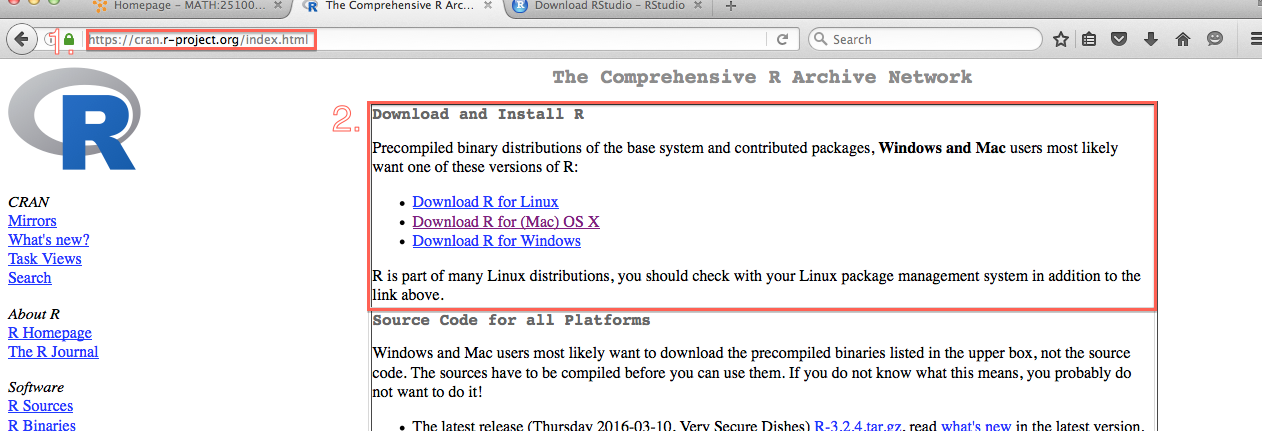
\includegraphics[width=\textwidth-1.65cm]{RInstall1.png}
\begin{enumerate}

\item Go to \url{http://cran.r-project.org}.

\item Follow the link for your operating system to the download page.

\vfill

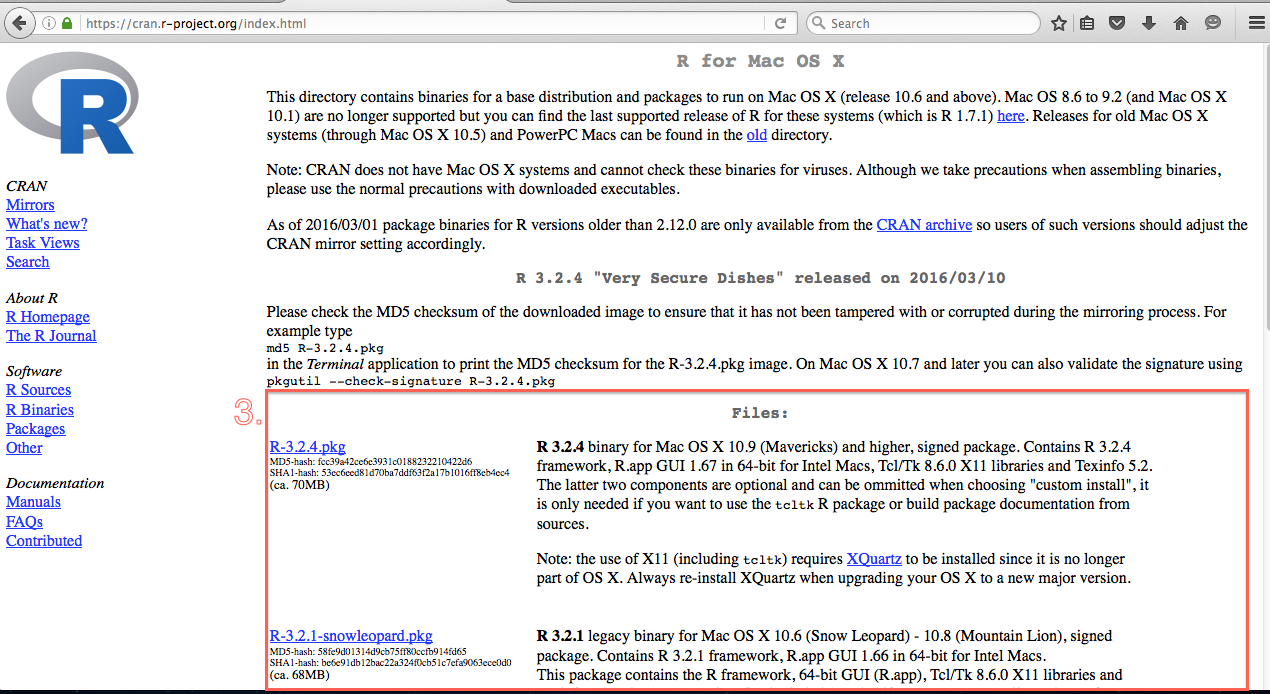
\includegraphics[width=\textwidth-1.65cm]{RInstall2.png}

\item Choose your operating system.

\vfill

\newpage

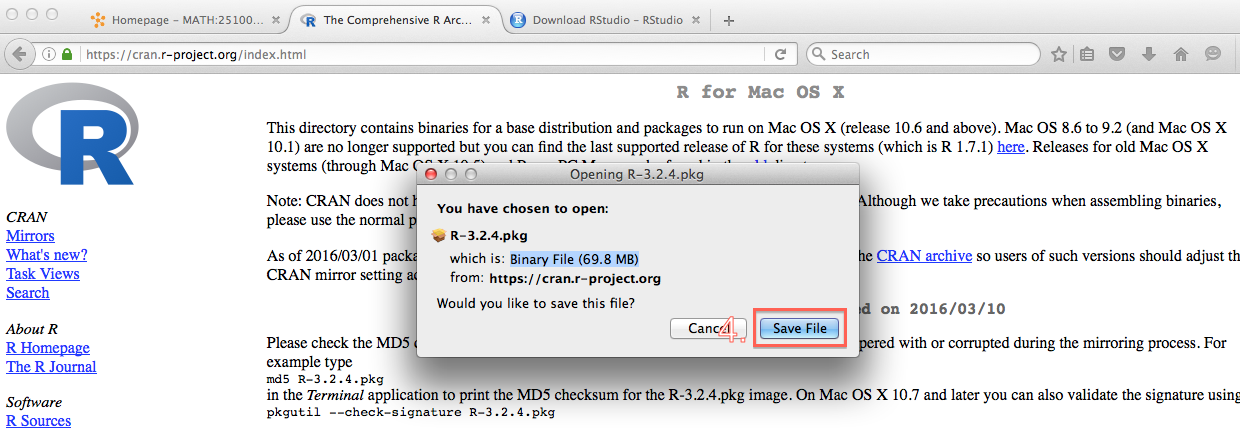
\includegraphics[width=\textwidth-1.65cm]{RInstall3.png}

\item Save and run the file.

\vfill

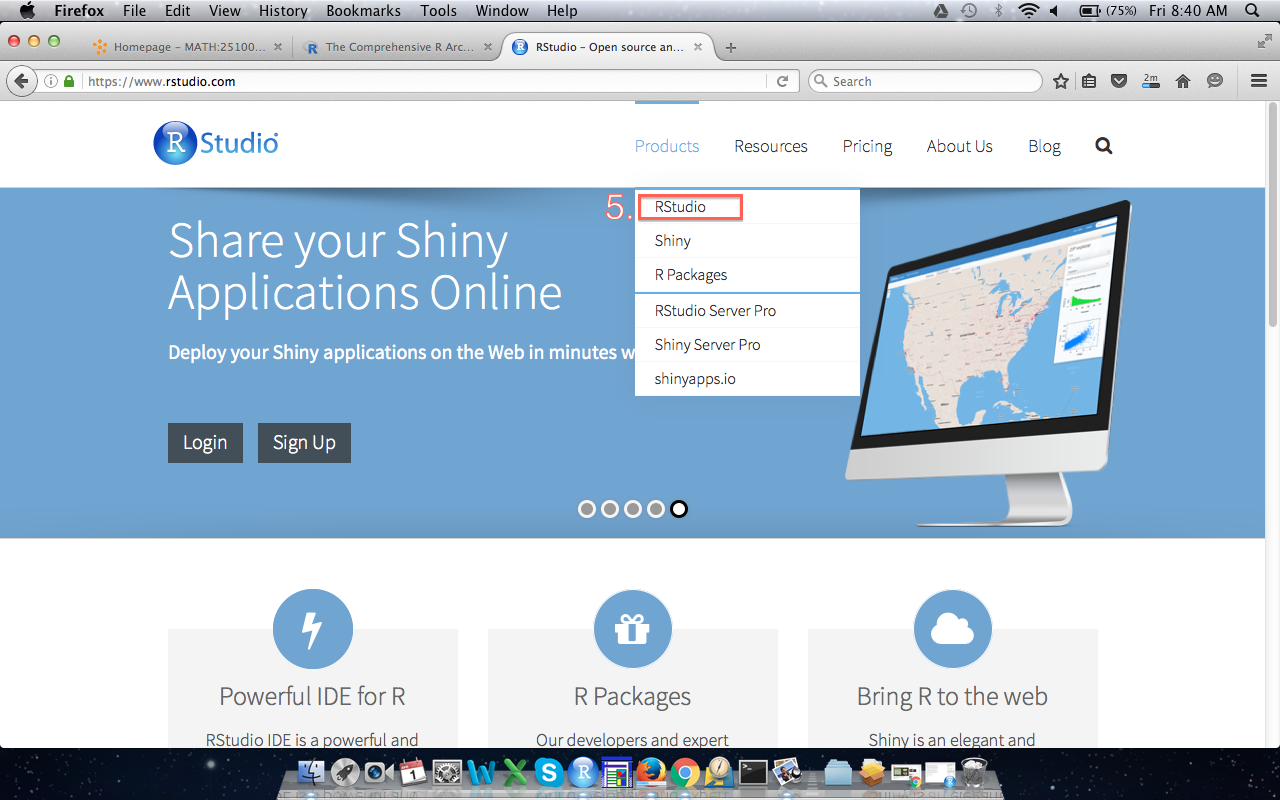
\includegraphics[width=\textwidth-1.65cm]{RInstall4.png}

\item Go to \url{http://www.rstudio.com} and under the ``Products" menu at the top, select RStudio.

\vfill

\newpage


\includegraphics[width=\textwidth-1.65cm]{RInstall5.png}

\item Follow the link under ``Desktop".

\vfill


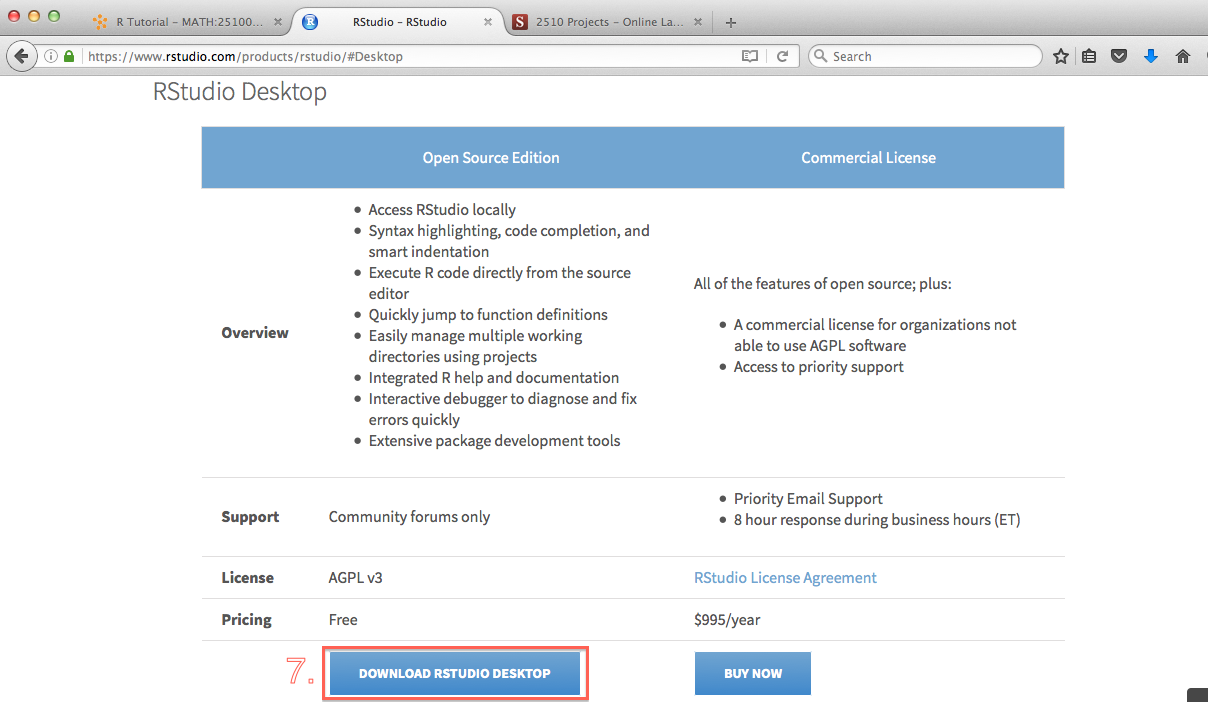
\includegraphics[width=\textwidth-1.65cm]{RInstall6.png}

\item Follow the ``Download RStudio Desktop" link.

\vfill

\newpage

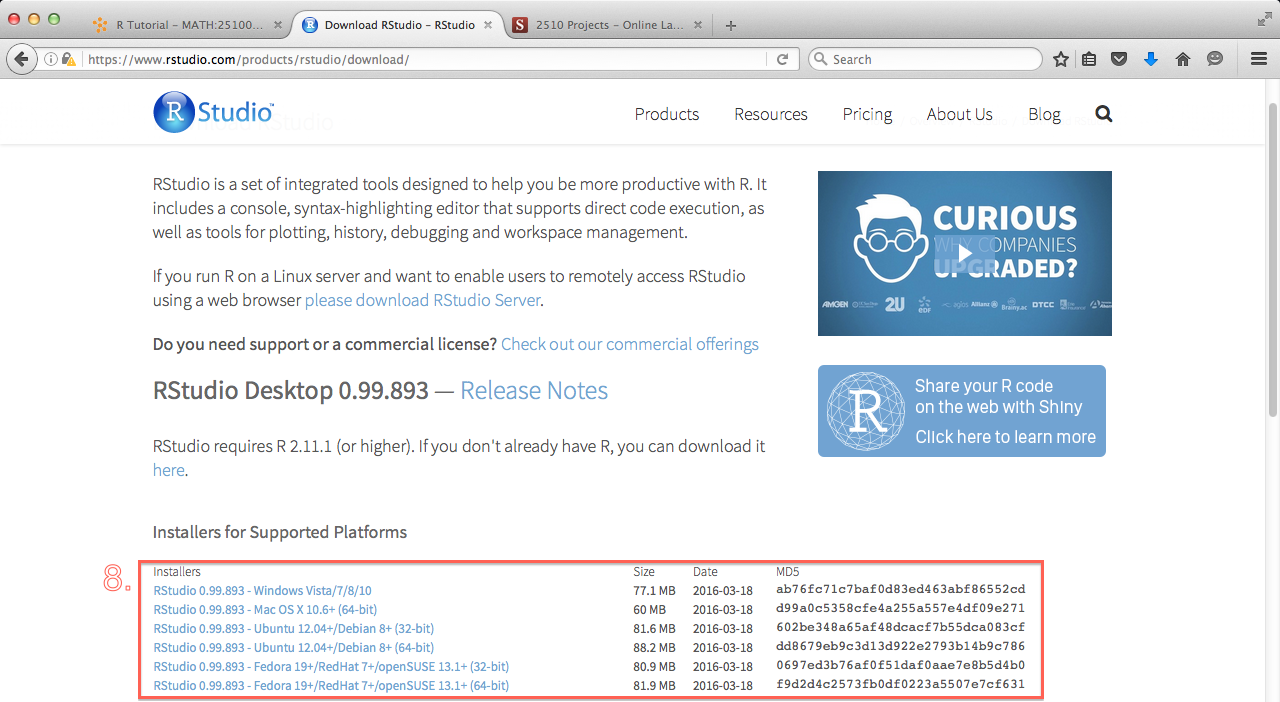
\includegraphics[width=\textwidth-1.65cm]{RInstall7.png}

\item Select your operating system and run the install file.

\end{enumerate}

\end{document}